\documentclass[conference,a4paper]{IEEEtran}

\usepackage{cite}
\usepackage{amsmath,amssymb,amsfonts}
\usepackage{graphicx}
\usepackage{booktabs}
\usepackage{textcomp}
\usepackage{xcolor}
\usepackage{url}

\newcommand{\SOtwo}{\mathrm{SO}(2)}
\newcommand{\Cfour}{C_4}

\title{What Rotation Equivariance Changes in Histopathology VAEs:\
Reconstruction, Label Efficiency, and Decoder Geometry}

\author{\IEEEauthorblockN{Anonymous Authors}}

\begin{document}

\maketitle

\begin{abstract}
Histopathology has abundant unlabeled image patches, scarce expert labels, and
no preferred tissue orientation. These properties motivate rotation-aware
self-supervised representations, but architectural equivariance does not by
itself guarantee better reconstructions, downstream performance, or a simple
latent pose coordinate. We compare two denoising variational autoencoders
(VAEs) trained on the same ovarian-cancer patches: a conventional convolutional
VAE and a continuous-rotation-equivariant $\SOtwo$ VAE. Both use a spatial
$16\times32\times32$ Gaussian latent and are frozen after 60,000 updates. We
evaluate reconstruction on 67,138 patches from 23 held-out whole-slide images
(WSIs), five-class WSI diagnosis, three-class tissue recognition under five
label budgets, and transformation consistency of the frozen latent-decoder
maps. The normal VAE has a slightly lower mean absolute reconstruction error,
but the paired WSI-bootstrap interval for the primary difference includes zero.
The $\SOtwo$ representation yields higher point estimates for WSI macro-F1
(0.483 vs. 0.389) and accuracy (0.609 vs. 0.522), without a conclusive macro-F1
interval. In tissue recognition, it is better at four low-label budgets, but
only 500 labels per class has a simultaneous interval excluding zero; the
highest budget favors the normal VAE. The strongest mechanistic result is more
specific: applying the prescribed spatial action to the $\SOtwo$ latent before
decoding realizes exact quarter-turn image rotations at approximately
$10^{-6}$ RMS error, while raw encoder posterior means are not strictly
equivariant. Thus, rotation-aware structure is clearly visible in the decoder,
yet it does not imply universal task improvement or content--pose
factorization. This endpoint-specific analysis provides a cautious template
for evaluating equivariant generative representations in digital pathology.
\end{abstract}

\begin{IEEEkeywords}
histopathology, variational autoencoder, rotation equivariance, $\SOtwo$,
whole-slide image classification, label efficiency
\end{IEEEkeywords}

\section{Introduction}

Whole-slide histopathology combines gigapixel images with labels that require
specialist review. Patch-based representation learning is therefore attractive:
large quantities of unlabeled tissue can train an encoder before a smaller
supervised model is fitted for diagnosis or tissue recognition
\cite{litjens_survey_2017,song_artificial_2023,tellez_neural_2021}. A second
property makes pathology a natural setting for symmetry-aware learning. Unlike
upright natural objects, many local tissue structures retain their biological
meaning after in-plane rotation.

Equivariant neural networks encode a transformation law rather than learning it
only from augmentation \cite{cohen_group_2016,cohen_steerable_2017}. Steerable
convolutions extend this principle to continuous planar rotations and
reflections \cite{weiler_general_2019}; rotation-equivariant classifiers have
also been studied directly in digital pathology \cite{veeling_rotation_2018}.
In principle, a correct inductive bias can reduce the number of examples needed
to learn a target function \cite{elesedy_provably_2021}. In practice, however,
three questions are often conflated:

\begin{enumerate}
    \item Does an equivariant autoencoder reconstruct unseen tissue better?
    \item Are its frozen representations more useful with limited labels?
    \item Where is the prescribed symmetry visible in a trained encoder--decoder?
\end{enumerate}

The questions are related but not equivalent. A decoder may commute with a
group action even when the encoder selects different representatives. A useful
downstream representation need not minimize pixel error. Conversely, a clean
architectural transformation law need not produce a low-dimensional latent
pose coordinate after training.

This work separates those claims in a matched experiment. We train a normal
convolutional denoising VAE and a repo-owned continuous-$\SOtwo$ steerable VAE
on the same $256\times256$ histopathology patches. The models share the data,
spatial latent shape, denoising objective, optimizer policy, update budget, and
evaluation splits. We then freeze both checkpoints and compare: (i) sealed
reconstruction, (ii) WSI diagnosis with the same multiple-instance learner,
(iii) tissue classification over nested label budgets, and (iv) exact and
interpolated rotation consistency. We additionally examine the decoder
pullback metric locally, because Euclidean latent differences can exaggerate
directions that barely affect the decoded image \cite{arvanitidis_latent_2018}.

Our contribution is not a claim that one model wins every endpoint. Instead, we
provide a controlled and statistically explicit account of where continuous
rotation structure helps, where it does not, and which equivariance claims are
actually supported by the frozen checkpoints.

\section{Related Work}

\subsection{Weakly Supervised Histopathology}

WSIs are commonly represented as bags of patch features because processing the
complete slide at native resolution is infeasible. Attention-based multiple
instance learning (MIL) learns a slide-level predictor from bag labels
\cite{ilse_attention_2018}, and later computational-pathology systems have
shown that such weak supervision can be data efficient
\cite{lu_data_2021}. Tellez \emph{et al.} demonstrated a complementary route:
learn an unsupervised compression model on image patches and use the resulting
codes for gigapixel prediction \cite{tellez_neural_2021}. Our evaluation follows
this two-stage logic, but holds the downstream learners fixed while changing
the frozen representation.

\subsection{Equivariance and Generative Representations}

For a group $G$, an encoder $E$, decoder $D$, input action $T_g$, and latent
action $\rho_g$, strict equivariance and decoder covariance are different
conditions:
\begin{align}
E(T_g x) &= \rho_g E(x), \label{eq:encoder-equivariance}\\
D(\rho_g z) &= T_g D(z). \label{eq:decoder-equivariance}
\end{align}
The first constrains the representative produced by the encoder; the second
constrains how a latent transforms when decoded. Group-equivariant and
steerable CNNs provide constructions for these transformation laws
\cite{cohen_group_2016,cohen_steerable_2017,weiler_general_2019}. VAEs provide
a probabilistic spatial representation through posterior parameters $\mu$ and
$\log\sigma^2$ and the reparameterization trick
\cite{kingma_auto_encoding_2014}. Our study evaluates both posterior and
decoded transformation behavior instead of treating architectural
equivariance as sufficient empirical evidence.

\section{Methods}

\subsection{Dataset and Split Discipline}

We use ovarian-cancer histopathology from the UBC-OCEAN resource
\cite{ubc_ocean_2023}. The unsupervised source contains 300,000 training and
30,000 validation patches from 322 and 39 non-TMA WSIs, respectively. Patches
are RGB, $256\times256$, and normalized to $[-1,1]$. The training corruption
changes hematoxylin/eosin stain coordinates and adds Gaussian noise with
probability 0.3. Twenty-five validation patches, five per source diagnosis,
were fixed before model comparison for visual and rotation analyses.

The sealed evaluation comprises 23 WSIs disjoint from the 106 training and 23
development WSIs used by downstream classifiers. It contains 67,138
foreground patches for reconstruction. The WSI task predicts five ovarian
diagnoses with supports 5/6/8/2/2. The tissue task uses 31,572 patches from the
same 23 WSIs: 21,796 tumor, 8,500 stroma, and 1,276 necrosis patches. Necrosis
occurs in only five WSIs. Sealed results were never used to select checkpoints,
architectures, label budgets, or stopping rules.

\subsection{Matched Variational Autoencoders}

Both VAEs map an input to spatial posterior parameters
$\mu,\log\sigma^2\in\mathbb{R}^{16\times32\times32}$ and decode a sampled
latent to RGB. They share 43 learned convolutions, the spatial schedule
$256\rightarrow128\rightarrow64\rightarrow32$, fixed anti-aliased
downsampling, bilinear upsampling followed by convolution, and a raw RGB output.
The objective is
\begin{equation}
\begin{aligned}
\mathcal{L}={}&\lVert \hat{x}-x\rVert_1
+0.1\bigl(1-\mathrm{SSIM}(\hat{x},x)\bigr)\\
&+\beta\,D_{\mathrm{KL}}(q_\phi(z\mid\tilde{x})\|\mathcal{N}(0,I)),
\end{aligned}
\end{equation}
with $\beta=0.01$ after warmup. AdamW, learning-rate scheduling, corruption,
training order, and the 60,000-update budget are matched.

The normal VAE uses ordinary convolutions, GroupNorm, and scalar gates. The
$\SOtwo$ VAE replaces these operations with continuous steerable convolutions,
field-aware normalization, and radial gates over scalar and first-order field
types. Its final posterior comprises 16 spatial scalar fields. The comparison
is intentionally capacity-conservative: the $\SOtwo$ model has 1,180,035
learned parameters versus 3,958,435 for the normal model (29.8\%). This avoids
giving the equivariant model more capacity, but it also means symmetry and
parameter count are not causally separated.

\begin{table}[t]
\caption{Frozen representation contract.}
\label{tab:contract}
\centering
\footnotesize
\begin{tabular}{lcc}
\toprule
Property & Normal VAE & $\SOtwo$ VAE \\
\midrule
Updates & 60,000 & 60,000 \\
Latent $\mu$ shape & $16\times32\times32$ & $16\times32\times32$ \\
Learned parameters & 3,958,435 & 1,180,035 \\
Training patches & 300,000 & 300,000 \\
Rotation constraint & none & continuous $\SOtwo$ \\
Downstream state & frozen $\mu$ & frozen $\mu$ \\
\bottomrule
\end{tabular}
\end{table}

\subsection{Downstream Evaluation}

For WSI diagnosis, every foreground patch is represented by deterministic
posterior $\mu$. The shared 1.51M-parameter MIL classifier first compresses each
latent map with a trainable convolutional patch encoder. Two local attention
blocks exchange information within a radius-two patch graph, while a learned
global stream summarizes the complete WSI for five-class prediction. The two
representation branches receive identical WSI membership, coordinate graphs,
initial classifier weights, epoch order, optimizer, and validation schedule.
Each branch independently selects its highest development macro-F1 checkpoint.

For tissue recognition, a smaller shared convolutional classifier predicts
tumor, stroma, or necrosis from frozen patch latents. We use nested,
class-balanced training subsets of 250, 500, 1,000, 2,500, and 5,671 labels per
class. Each budget begins from identical weights for both representations.
Natural-distribution validation selects the checkpoint; the complete sealed
test distribution is evaluated once.

\subsection{Reconstruction and Rotation Geometry}

Reconstruction is evaluated with MAE and MSE in the normalized domain and with
PSNR and SSIM after clamping to $[0,1]$. The primary endpoint is mean MAE.

For rotations, let $R_k$ be an exact array rotation by $90k$ degrees and let
$\rho_k$ rotate every spatial latent channel in the same way. We distinguish
the encoded cycle $e_k=E_\mu(R_kx)$ from the prescribed cycle
$a_k=\rho_kE_\mu(x)$. The decoder-action error is
\begin{equation}
\epsilon_D(k,x)=\operatorname{RMS}\!\left[D(a_k)-R_kD(e_0)\right].
\end{equation}
We also use an interpolated $0,5,\ldots,355$ degree sweep. Its normalized action
ratio divides the action error by the error produced when the latent is left
untransformed; 1 is the no-action baseline. The canonicalization ratio similarly
compares $D(\rho_{-\theta}E_\mu(R_\theta x))$ with $D(E_\mu(x))$ relative to
leaving the rotated embedding unchanged. A preregistered absolute target of
0.5 asks whether the action removes at least half of the baseline error.

Finally, at fixed validation ranks 0 and 12 we estimate the local decoder
pullback $G(z)=J_D(z)^\top J_D(z)$ without materializing the Jacobian. Direct
JVP/VJP products and stochastic Lanczos quadrature with 64 probes and depth 64
estimate the trace and dimensions required for 95\% and 99\% spectral mass.
This is a two-anchor diagnostic, not a population estimate or proof of a global
manifold.

\subsection{Uncertainty and Claim Boundaries}

Reconstruction differences use 10,000 paired WSI-cluster bootstrap replicates;
patch standard deviations describe dispersion only. WSI diagnosis uses a
diagnosis-stratified paired bootstrap over 23 WSIs. Tissue differences use a
WSI bootstrap stratified by observed tissue support and simultaneous 95\%
intervals across the five label budgets. These intervals do not cover new VAE
or classifier training seeds. Rotation analyses use the fixed validation set;
their WSI-resampled intervals are descriptive and do not support population
inference.

\section{Results}

\subsection{Reconstruction Fidelity}

Both models preserve the major tissue structures and staining patterns on the
same predetermined validation patches (Fig.~\ref{fig:reconstructions}). On the
sealed set, the normal VAE has slightly better point estimates for all four
reconstruction metrics (Table~\ref{tab:reconstruction}). Primary MAE is
0.062872 for normal and 0.064230 for $\SOtwo$. The paired difference
normal-minus-$\SOtwo$ is $-0.001358$, with 95\% CI
$[-0.002213,0.000046]$. Because the interval includes zero, the primary
reconstruction difference is not established. PSNR and SSIM favor the normal
model descriptively, but remain secondary endpoints.

\begin{figure*}[t]
\centering
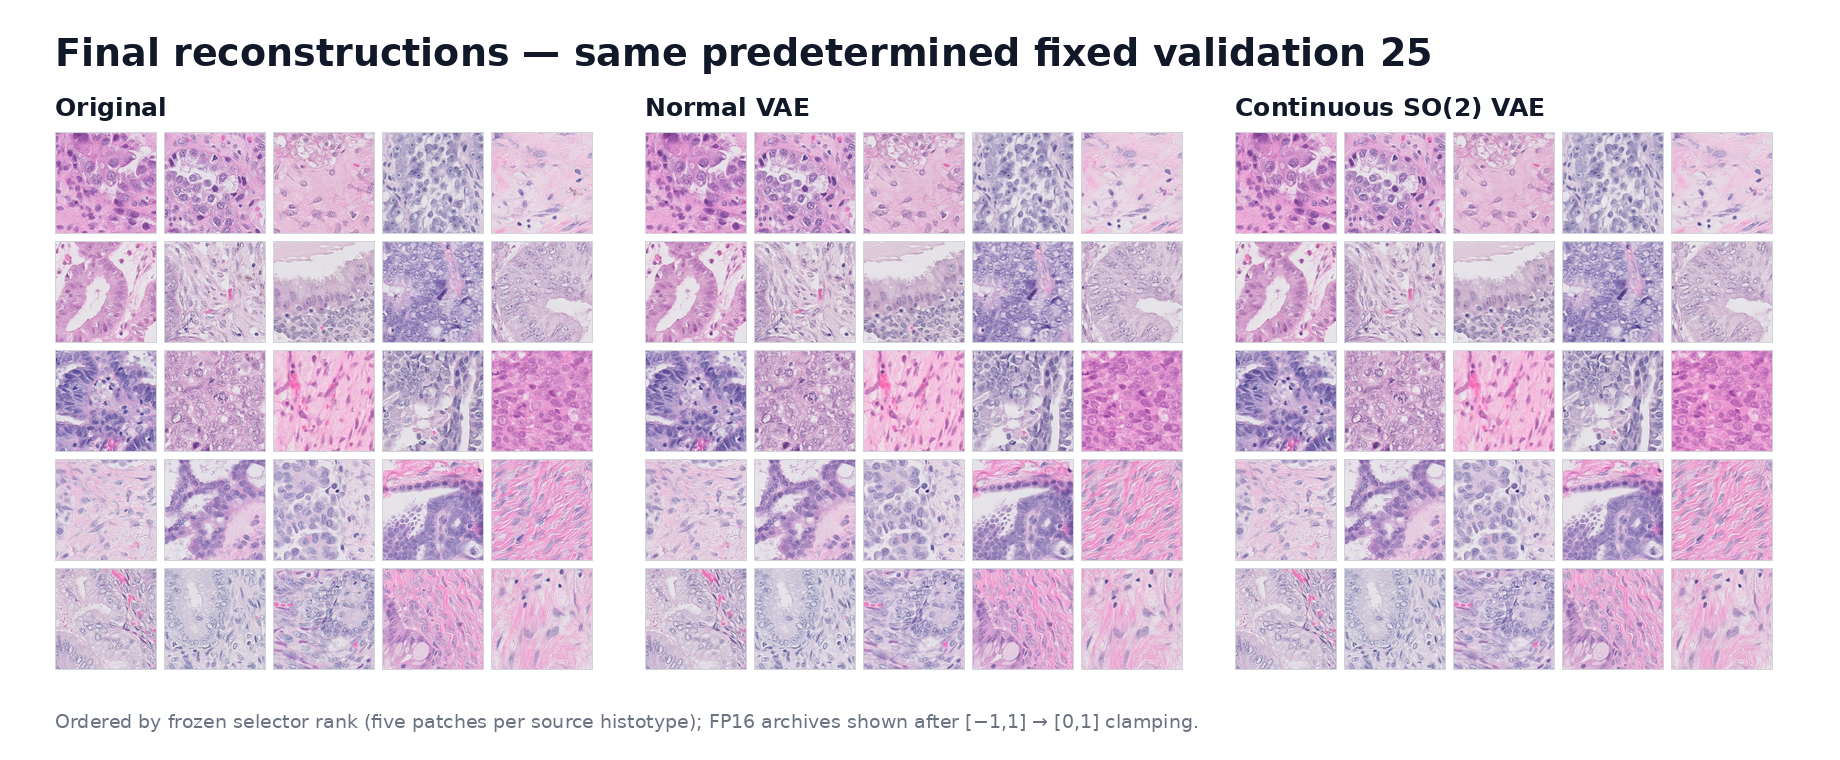
\includegraphics[width=0.96\textwidth]{figures/reconstructions_fixed25.png}
\caption{Originals and final reconstructions for the same 25 validation
patches fixed before analysis. Visual inspection is descriptive; the sealed
quantitative evaluation uses 67,138 patches from 23 WSIs.}
\label{fig:reconstructions}
\end{figure*}

\begin{table}[t]
\caption{Sealed reconstruction over 67,138 patches. Values are mean
(population SD).}
\label{tab:reconstruction}
\centering
\footnotesize
\begin{tabular}{lcc}
\toprule
Metric & Normal VAE & $\SOtwo$ VAE \\
\midrule
MAE $\downarrow$ & 0.0629 (0.0239) & 0.0642 (0.0223) \\
MSE $\downarrow$ & 0.0080 (0.0074) & 0.0083 (0.0067) \\
PSNR dB $\uparrow$ & 27.923 (2.721) & 27.658 (2.595) \\
SSIM $\uparrow$ & 0.7575 (0.0842) & 0.7436 (0.0862) \\
\bottomrule
\end{tabular}
\end{table}

\subsection{WSI Diagnosis and Tissue Label Efficiency}

On 23 sealed WSIs, $\SOtwo$ has higher point estimates for macro-F1 and
accuracy, while balanced accuracy is essentially unchanged
(Fig.~\ref{fig:downstream}). Macro-F1 is 0.483 versus 0.389, but the 95\%
interval for normal-minus-$\SOtwo$, $[-0.207,0.050]$, includes zero. Accuracy
is 0.609 versus 0.522 with interval $[-0.217,0.043]$. Mean cross-entropy is
lower for $\SOtwo$ (0.993 versus 1.323), and its paired interval favors
$\SOtwo$; this is a secondary endpoint. Class-level conclusions are fragile:
LGSC and MC contain only two WSIs each, and the two models fail on different
rare classes.

The tissue task reveals a non-monotone interaction with label budget.
$\SOtwo$ has higher macro-F1 at 250, 500, 1,000, and 2,500 labels per class.
Only the 500-label difference has a simultaneous interval excluding zero:
normal-minus-$\SOtwo=-0.064$, 95\% simultaneous CI
$[-0.121,-0.008]$. At 5,671 labels per class, the normal representation is
higher (0.766 versus 0.710), although the simultaneous interval nearly touches
zero. The normalized area under the log-budget learning curve is 0.615 for
normal and 0.631 for $\SOtwo$; its simultaneous difference interval includes
zero. Therefore, the results support one budget-specific low-label advantage,
not universal sample-efficiency dominance.

\begin{figure*}[t]
\centering
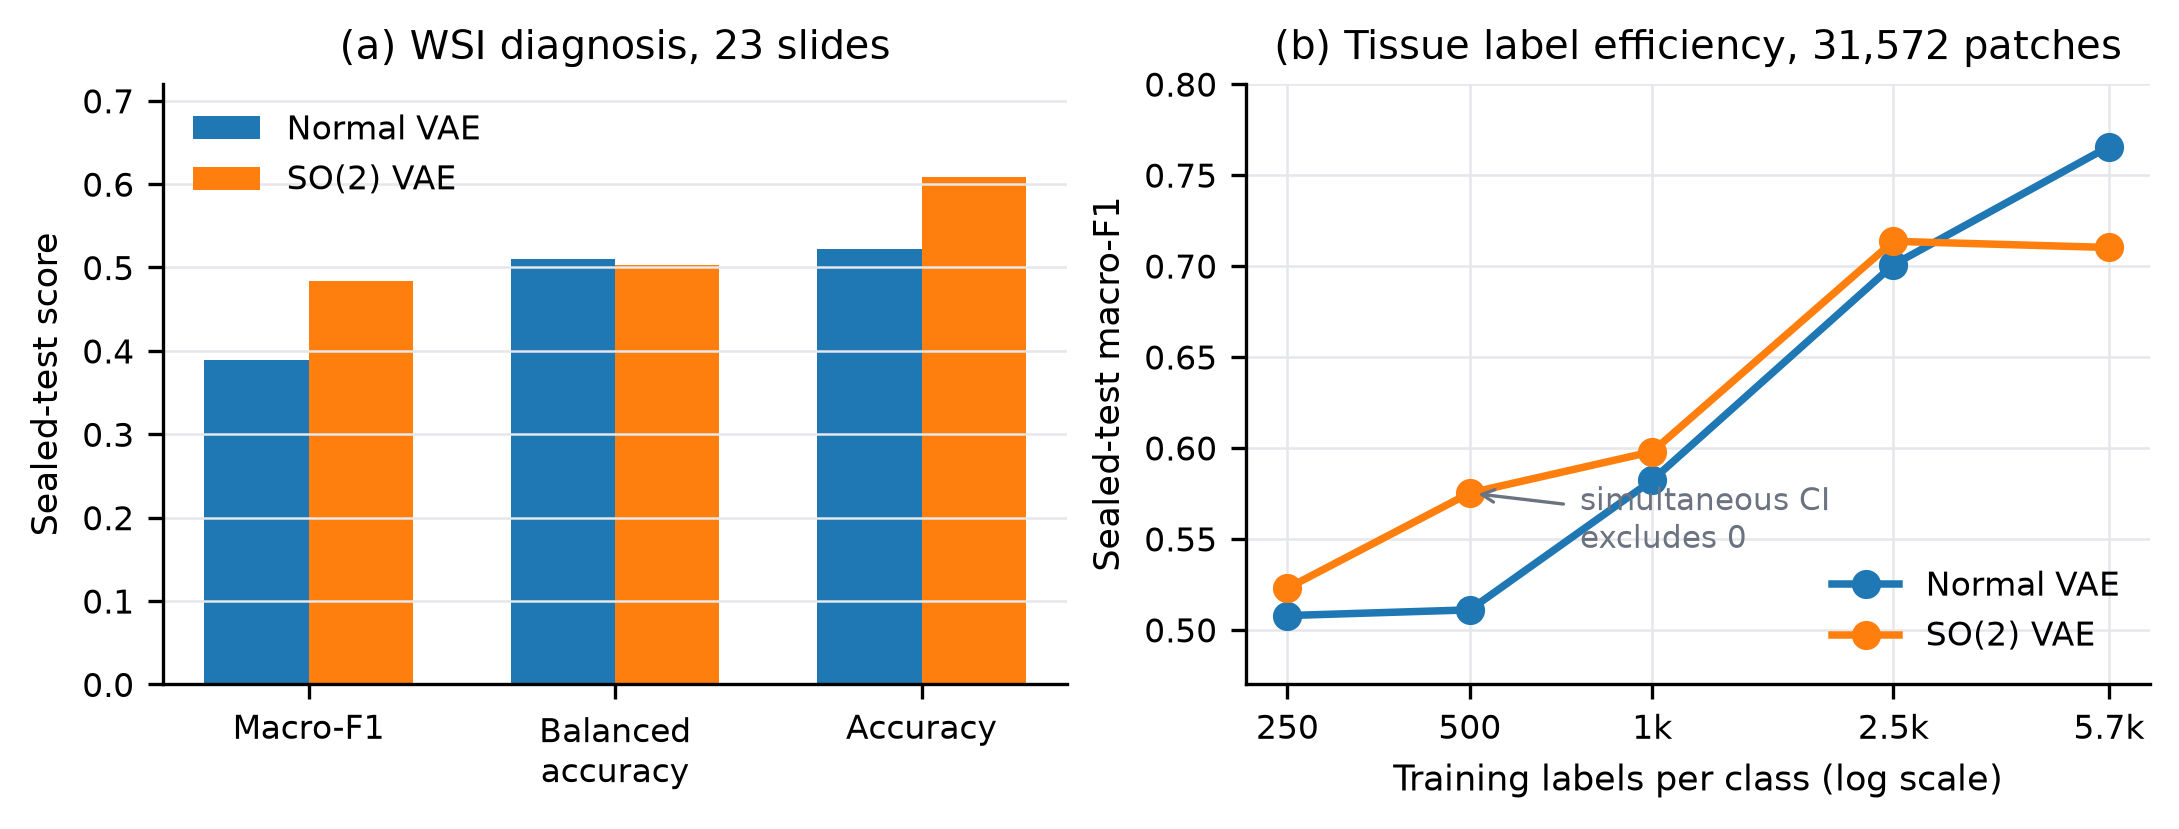
\includegraphics[width=0.94\textwidth]{figures/downstream_results.png}
\caption{Frozen-representation downstream results. (a) WSI diagnosis point
estimates on 23 sealed slides. (b) Tissue macro-F1 on 31,572 sealed patches;
training subsets are nested and class balanced. Only 500 labels per class has
a simultaneous difference interval excluding zero.}
\label{fig:downstream}
\end{figure*}

\begin{table}[t]
\caption{Sealed downstream macro-F1. Tissue intervals are simultaneous across
budgets and are reported for normal-minus-$\SOtwo$.}
\label{tab:downstream}
\centering
\footnotesize
\begin{tabular}{lccc}
\toprule
Task/budget & Normal & $\SOtwo$ & Difference CI \\
\midrule
WSI diagnosis & 0.389 & 0.483 & $[-0.207,0.050]$ \\
Tissue 250 & 0.508 & 0.523 & $[-0.072,0.041]$ \\
Tissue 500 & 0.511 & 0.575 & $[-0.121,-0.008]$ \\
Tissue 1,000 & 0.582 & 0.598 & $[-0.072,0.041]$ \\
Tissue 2,500 & 0.701 & 0.714 & $[-0.069,0.044]$ \\
Tissue 5,671 & 0.766 & 0.710 & $[-0.001,0.112]$ \\
\bottomrule
\end{tabular}
\end{table}

\subsection{Decoder Equivariance Is Stronger Than Encoder Equivariance}

The dense interpolated sweep favors $\SOtwo$ consistently in route
agreement. Median decoded-action ratios are 0.550 for $\SOtwo$ and 0.713 for
normal; canonicalization ratios are 0.513 and 0.661. The $\SOtwo$ value is
lower on all 25 paired patches for both metrics, and the WSI-resampled
descriptive intervals for the paired median differences exclude zero. However,
the $\SOtwo$ medians remain just above the absolute 0.5 target, so this dense
interpolation experiment does not by itself verify exact continuous
equivariance.

The exact quarter-turn control is qualitatively different. At 90, 180, and
270 degrees, the prescribed latent action of the $\SOtwo$ checkpoint commutes
with decoding at approximately $10^{-6}$ image RMS, compared with normal-VAE
medians of 0.165--0.190. The corresponding normalized action ratio aggregates
to $2.18\times10^{-6}$ for $\SOtwo$ and 0.709 for normal. This verifies a
shared, parameter-free $\Cfour$ decoder action on all 25 fixed patches
(Fig.~\ref{fig:decoder-geometry}). It does not verify all continuous angles,
encoder equivariance, reflections, or complete $D_4/O(2)$ symmetry.

Indeed, raw posterior behavior is less favorable. For exact quarter-turns, the
relative discrepancies between $E_\mu(R_kx)$ and $\rho_kE_\mu(x)$ are not lower
for $\SOtwo$. Thus, Eqs.~\eqref{eq:encoder-equivariance} and
\eqref{eq:decoder-equivariance} must not be merged: the decoder realizes the
prescribed cardinal action while the encoder posterior mean can select a
different latent representative.

\begin{figure*}[t]
\centering
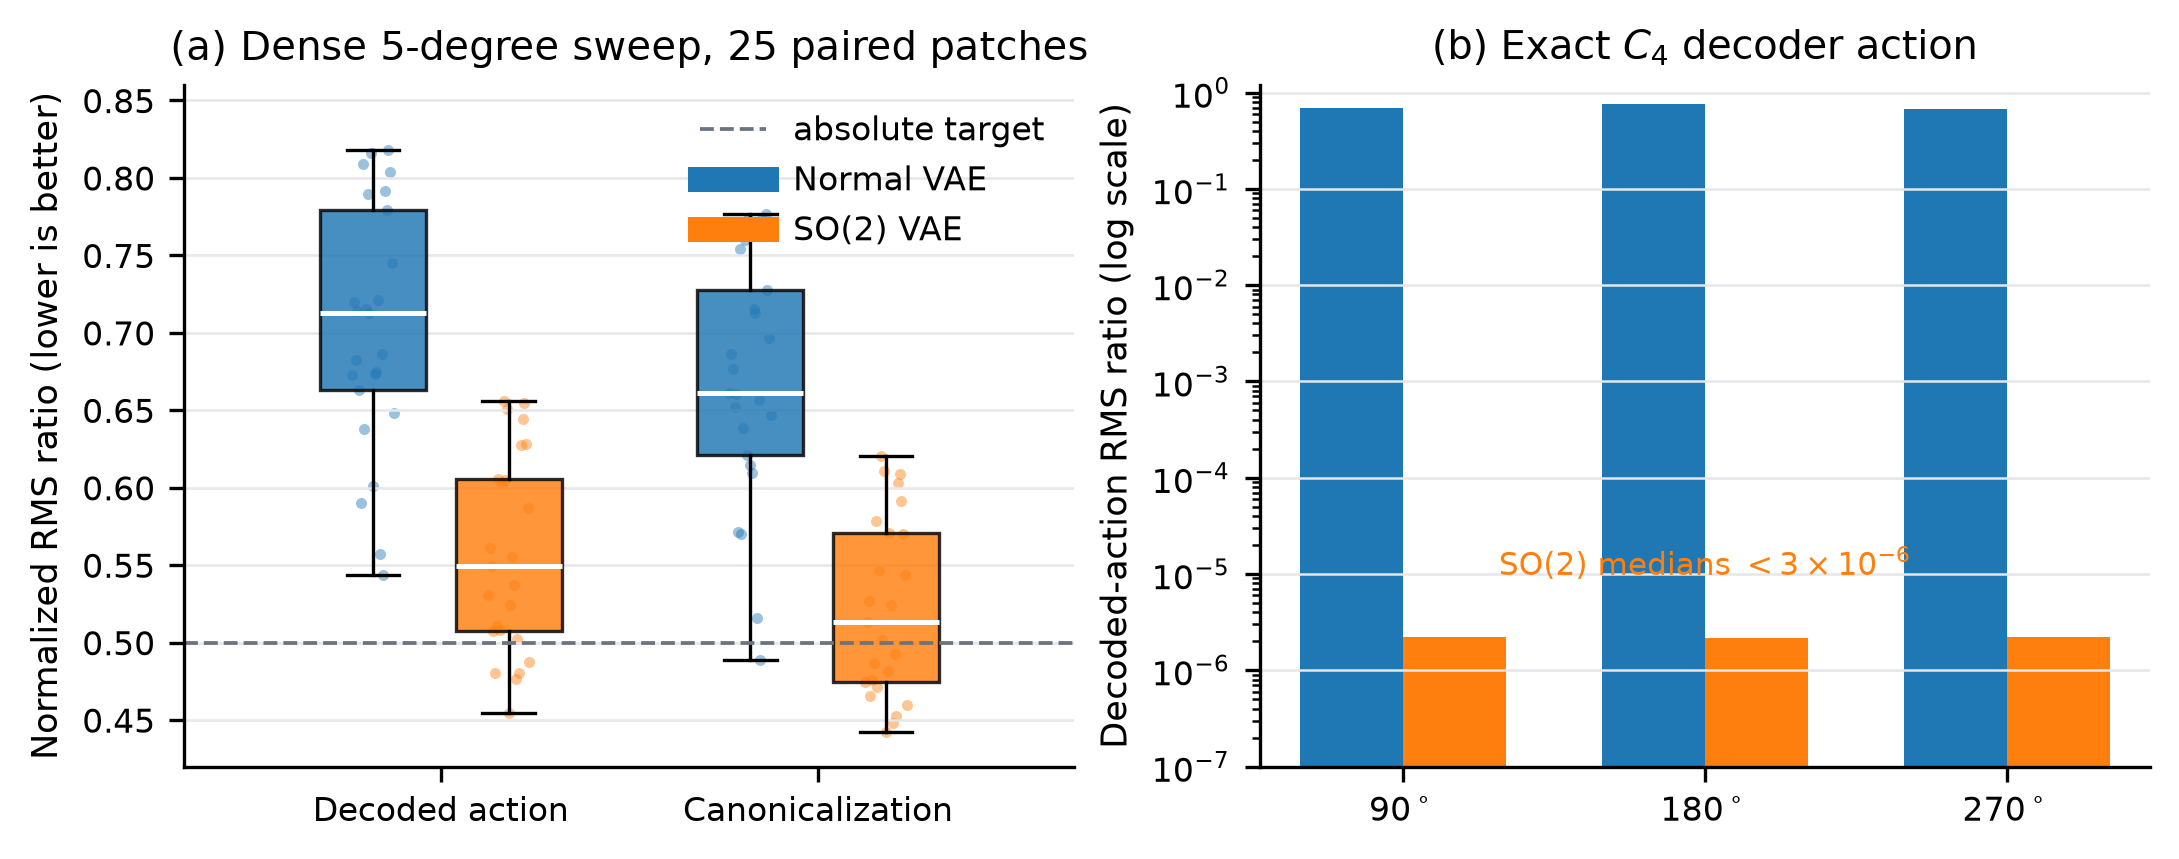
\includegraphics[width=0.94\textwidth]{figures/decoder_geometry.png}
\caption{Transformation consistency on the fixed validation set. (a)
Interpolated 5-degree sweep; lower normalized RMS ratios indicate better route
agreement, and 0.5 is the preregistered absolute target. (b) Exact cardinal
rotations on a logarithmic scale. The $\SOtwo$ decoder realizes the prescribed
$\Cfour$ action almost exactly.}
\label{fig:decoder-geometry}
\end{figure*}

\subsection{Local Decoder-Visible Geometry}

The pullback analysis supports a narrower claim about decoder-visible
complexity. Across ranks 0 and 12 and four exact angles, the estimated
$\SOtwo$/normal trace ratio ranges from 0.895 to 0.959. The $\SOtwo$ estimate
also requires fewer dimensions to reach both 95\% and 99\% spectral mass in
all eight matched states. At rank 0, normal $d_{95}$ ranges 4,886--4,928 while
$\SOtwo$ ranges 4,565--4,581; at rank 12, the ranges are 3,835--4,036 and
3,726--3,750. These observations are consistent with a somewhat more compact
local decoder-visible spectrum, but they come from only two anchors. They do
not establish a population effect, a continuous rotation orbit, a global
quotient, or low-dimensional disentanglement.

\begin{table*}[t]
\caption{Evidence map. Each conclusion is intentionally limited to the
measurement that supports it.}
\label{tab:evidence-map}
\centering
\footnotesize
\begin{tabular}{p{0.19\textwidth}p{0.35\textwidth}p{0.38\textwidth}}
\toprule
Question & Main evidence & Supported conclusion \\
\midrule
Reconstruction fidelity & 67,138 sealed patches; WSI-cluster bootstrap &
Normal is descriptively better; the primary MAE difference is not established. \\
WSI representation utility & 23 sealed WSIs under one shared MIL contract &
$\SOtwo$ has favorable point estimates, without a conclusive macro-F1 interval. \\
Low-label tissue utility & Five nested budgets with simultaneous intervals &
One supported advantage at 500 labels/class; no global sample-efficiency claim. \\
Decoder rotation action & Fixed-25 exact quarter-turn control &
The $\SOtwo$ decoder realizes the prescribed $\Cfour$ action near numerical precision. \\
Encoder equivariance & $E_\mu(R_kx)$ versus $\rho_kE_\mu(x)$ &
Strict equivariance of the final posterior mean is not supported. \\
Continuous/content--pose geometry & Dense interpolation and shared-action probes &
No verified continuous action, global quotient, or content--pose factorization. \\
\bottomrule
\end{tabular}
\end{table*}

\section{Discussion}

The results separate three effects that would be obscured by a single summary
score. First, the normal VAE retains a small descriptive reconstruction
advantage. The primary interval crosses zero, but the consistent secondary
metrics warn against assuming that stronger architectural structure must
improve pixel fidelity.

Second, the $\SOtwo$ representation shows promising but uneven downstream
behavior. Its WSI point estimates are better for macro-F1 and accuracy, and it
has a clear simultaneous advantage at one low-label tissue budget. Yet these
signals do not persist at the highest tissue budget, and the global learning
curve comparison is inconclusive. This pattern is compatible with an inductive
bias that can help in a restricted low-data regime, but one training seed and
23 test WSIs cannot isolate that mechanism.

Third, the most decisive evidence is mechanistic rather than task-level. The
$\SOtwo$ decoder realizes the prescribed exact $\Cfour$ spatial action nearly
perfectly. At the same time, the raw posterior mean does not satisfy the same
strict encoder relation, dense interpolated ratios miss the absolute target,
and previous low-dimensional shared-action probes fail to outperform identity.
Consequently, the correct interpretation is not that the learned latent equals
``content times angle.'' A more conservative interpretation is that the
decoder contains a coherent cardinal rotation mechanism while the encoder may
choose different representatives in a high-dimensional, decoder-redundant
space.

The parameter count deserves equal emphasis. The $\SOtwo$ VAE uses only 29.8\%
of the parameters of the normal VAE. This is an efficiency result, but also a
causal confound: any difference may reflect symmetry, capacity, optimization,
or their interaction. Our study therefore supports endpoint-specific
comparison between these frozen checkpoints, not attribution to symmetry alone.

\section{Limitations}

The study has one training trajectory per VAE and one downstream trajectory per
representation and budget. Bootstrap intervals measure sampling variation
across observed WSIs, not initialization or training-seed uncertainty. The WSI
test contains 23 slides, with only two examples in each of two diagnoses.
Tissue evaluation contains many patches but only 23 biological clusters, and
necrosis appears in five.

The reconstruction aggregation and bootstrap were finalized after later test
labels had been opened, although neither VAE checkpoint was changed. Rotation
geometry is post-hoc validation-only analysis on 25 fixed patches. Interpolated
angles depend on bilinear resampling and do not inherit the numerical exactness
of array quarter-turns. Pullback spectra cover two anchors only. Finally, the
models differ substantially in parameter count, so the experiment does not
identify the causal effect of equivariance independently of capacity.

\newpage
\section{Conclusion}

A continuous-$\SOtwo$ VAE can expose meaningful rotation structure without
winning every conventional endpoint. Here, the normal VAE reconstructs slightly
better descriptively; the $\SOtwo$ representation has favorable but uncertain
WSI results and one simultaneous low-label tissue advantage; and its decoder
realizes exact cardinal rotations with near-numerical precision. Raw posterior
means do not support strict encoder equivariance or a simple content--pose
factorization. Evaluations should therefore report reconstruction, downstream
utility, and transformation mechanism separately.

\IEEEtriggeratref{4}
\bibliographystyle{IEEEtran}
\bibliography{references}

\end{document}
